\documentclass{article}
\usepackage[margin=1.25in]{geometry}
\usepackage{amsmath, amssymb, setspace, enumerate, enumitem}
\usepackage{setspace}
\usepackage{graphicx}
\doublespacing

\begin{document}
    \begin{enumerate}[label=\textbf(Q1)]
        \item is $4^{1536} \equiv 9^{4824}\ mod\ 35$\\
        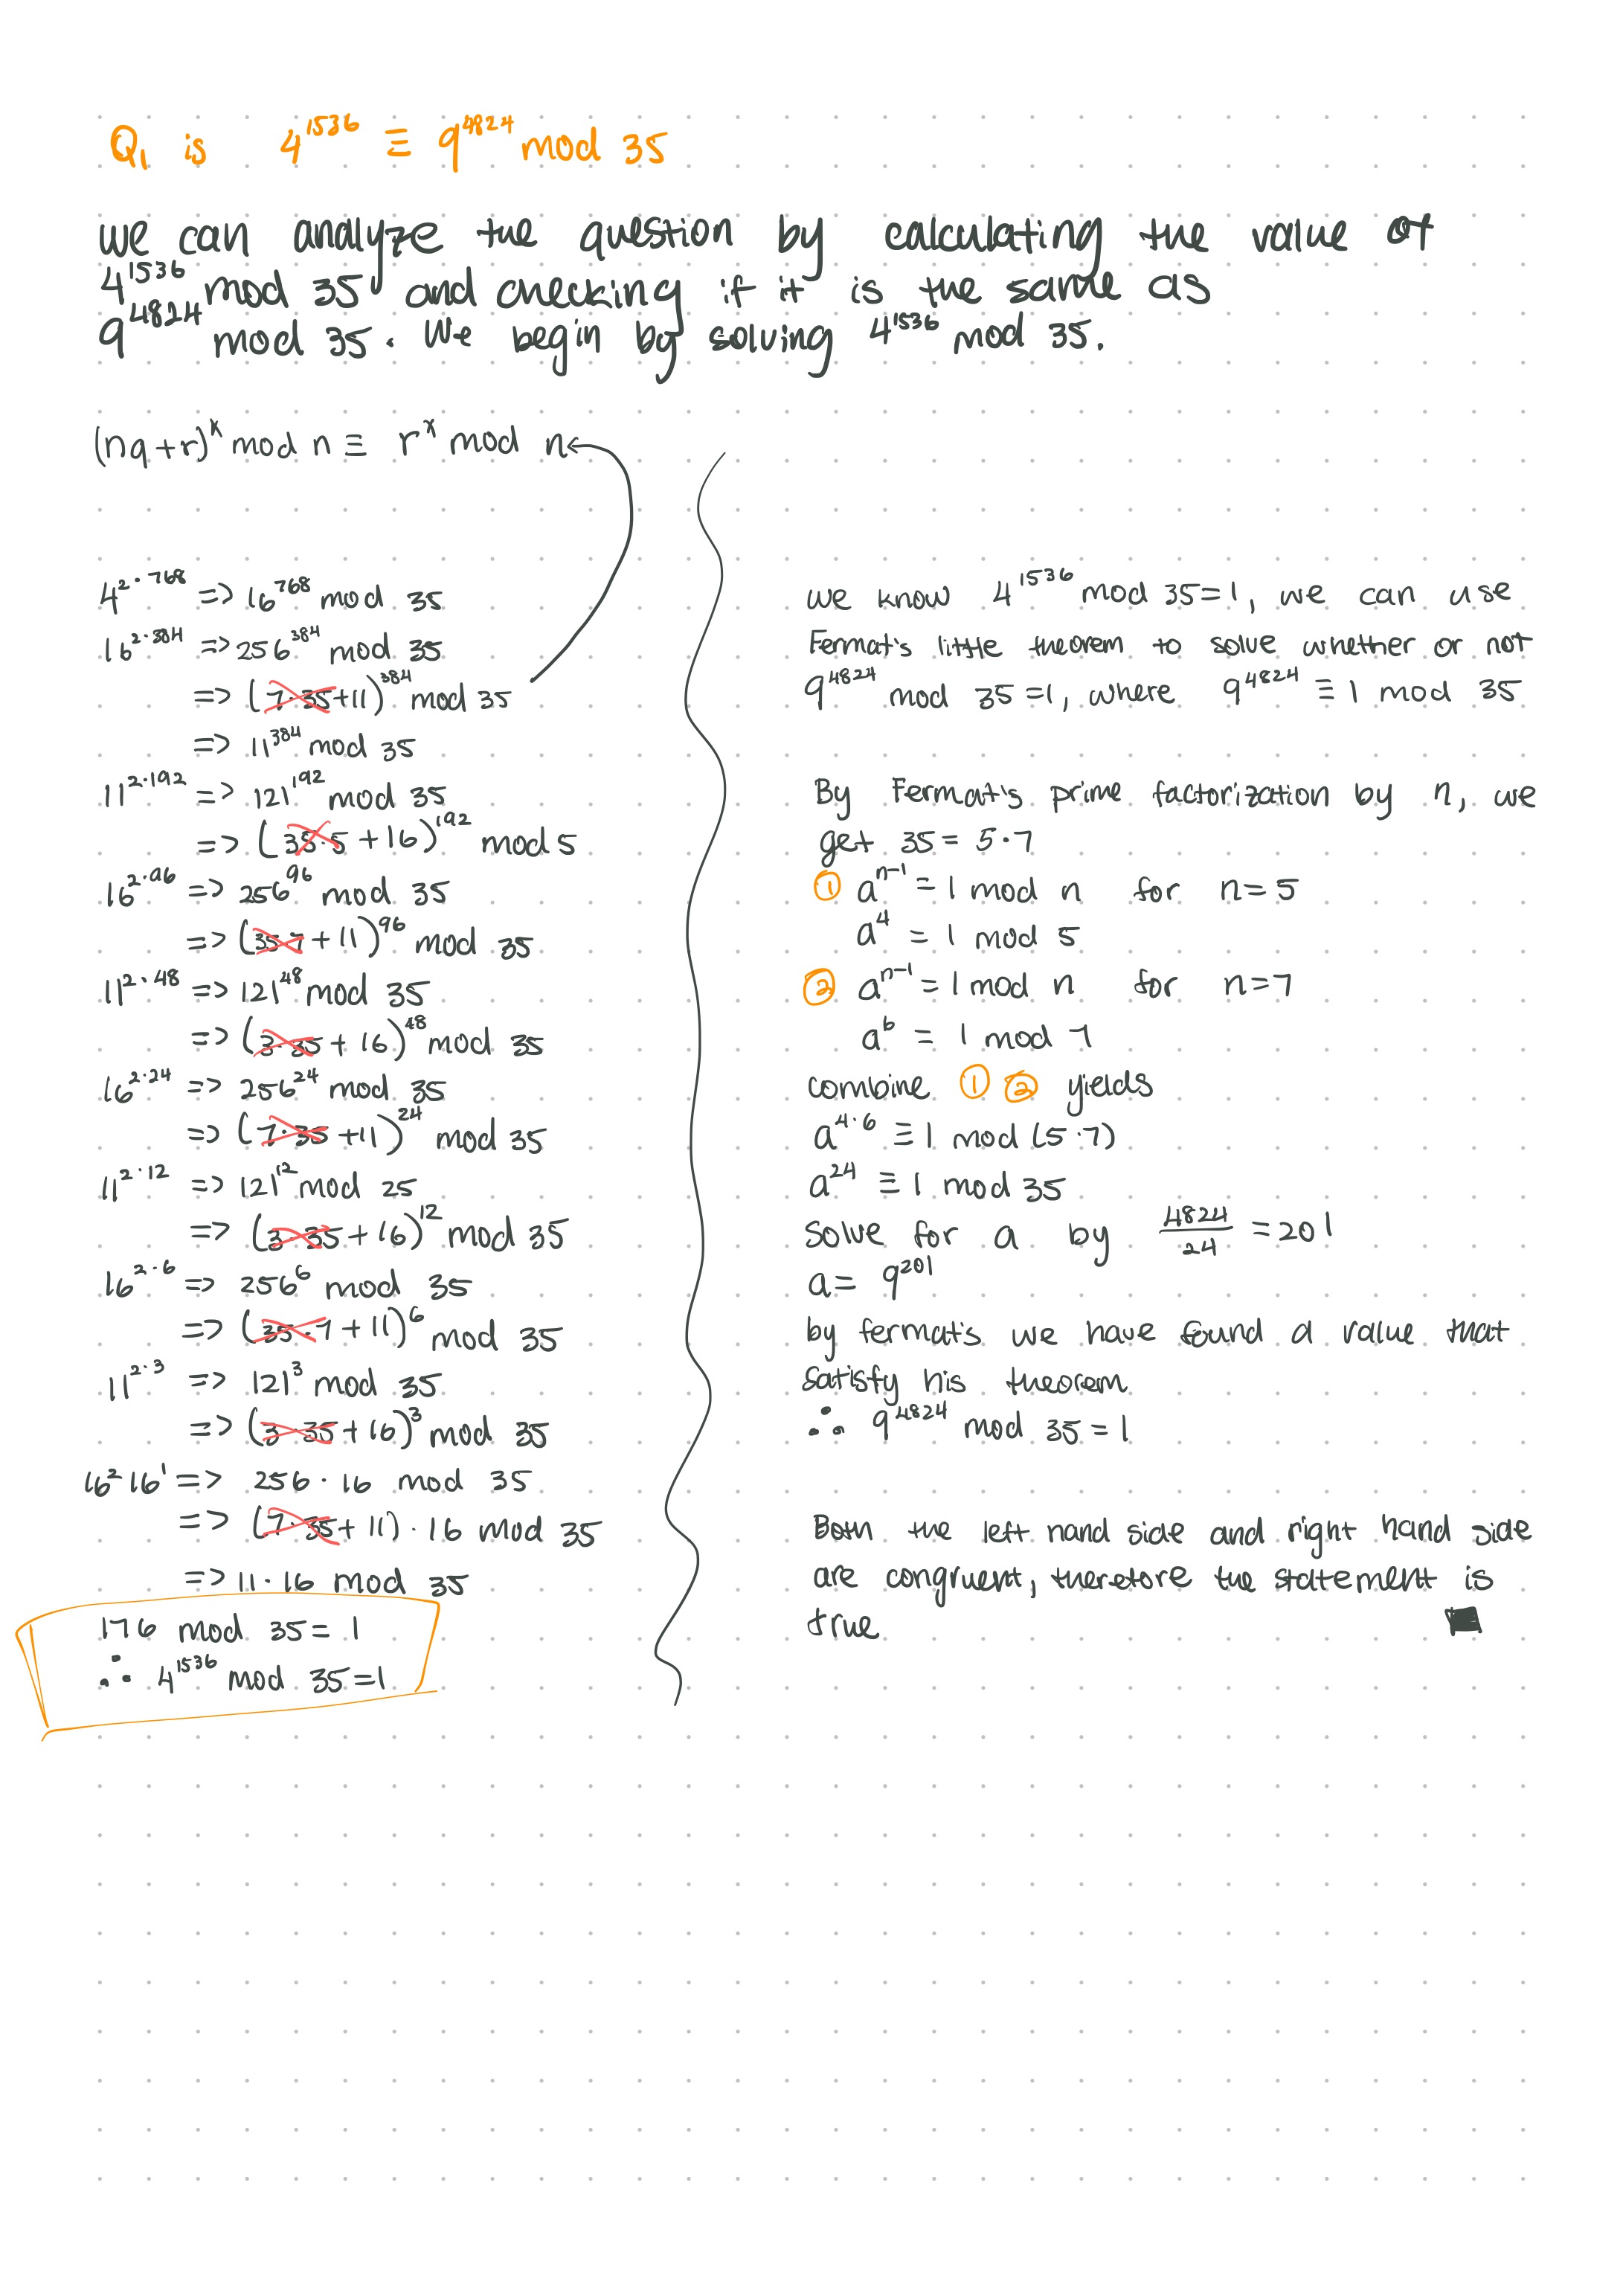
\includegraphics[scale=0.20, trim={0 20cm 0 0}, clip]{q1.jpg}
    \end{enumerate}
    \pagebreak
    \begin{enumerate}[label=\textbf{Q2}]
        \item Solve $x^{86} \equiv 6\ mod\ 29$
    \end{enumerate}
    \pagebreak
    \begin{enumerate}[label=\textbf{Q3}]
        \item Prove that $gcd(F_{n+1},\ F_n) = 1$, for $n \geq 1$, where $F_n$
        is the n-th Fibonacci element.\\
        \textbf{Solution: }\\
        When the $gcd$ of two numbers is 1, that means that the numbers are
        relatively prime, meaning that there is no number $n \neq 1$ that divides
        both of the numbers. We can prove the following statement by induction.\\
        \textbf{Base case:}\\
        For $n = 0$, we check the $gcd(F_0, F_1)$, which are $gcd(1, 1)$, these two
        numbers satisfy as $gcd(1,1) = 1\ \checkmark$\\
        \textbf{Induction step:}\\
        For our induction hypothesis, we assume that $gcd(F_n, F_{n+1}) = 1$. We must
        prove that the statement is true as well for $n = k + 1$ and prove $gcd(F_{k+1}, F_{k+2}) = z$,
        for $z = 1$\\
        By the equation, we know that $z \mid F_{k+1}$, $z \mid F_{k+2}$ and $z \mid F_{k} + F_{k+1}$
        since $F_x = F_{x - 2} + F_{x - 1}$ for $x \in \mathbb{N}$. $z \mid F_k + F{k+1}$ tells us that
        $z \mid F_k$ and $z \mid F_{k+1}$, we can derive Euclid's GCD by stating $gcd(F_k, F_{k+1}) = z$.
        From our induction hypothesis, we know that $gcd(F_n, F_{n+1}) = 1$, therefore, $z$ is also $1$.
        We prove the following claim by a direct proof via induction. $\hfill \blacksquare$
        
    \end{enumerate}
\end{document}